% Video4Real (ECCV 2026 workshop) extended abstract.
% The official call states that accepted abstracts are excluded from the ECCV
% workshop proceedings: https://sites.google.com/utwente.nl/video4real/home
% Uses the vendored ECCV 2026 template pinned in paper/eccv2026/PINNED.txt
% (da8c09c40239d5665757527e77388f4716a6564a).
% Verified with TeX Live 2025 on 2026-07-28: seven PDF pages; references
% begin on PDF page 6, within the seven-page limit excluding references.
%
% Build from the repository root with `make video4real`.
% Submission ID 12. The `review' option anonymizes
% authors/institute/running heads automatically (double-blind).
\documentclass[runningheads]{llncs}

% Use the pinned package even if a local shadow copy exists beside this source.
\usepackage{silence}
\WarningFilter{latex}{You have requested package}
\usepackage[review,year=2026,ID=12]{eccv2026/eccv} % double-blind review version
\usepackage[pagebackref,breaklinks,colorlinks]{hyperref}
\usepackage{graphicx}
\usepackage{booktabs}
\usepackage{placeins}
\hypersetup{pdfauthor={},pdftitle={},pdfsubject={},pdfkeywords={}}

\graphicspath{{figures/}{../figures/}}

% HDD global paired encoder-seq-DTW minus BoT CI (job 9654434, verbatim from JSON).
\newcommand{\hddGlobalDtwBot}{$-0.079$ $[-0.106, -0.062]$}

\title{When Conditional Sequence Matching Does Not Transfer to Global Video Retrieval}

% Anonymized automatically by the eccv `review' option; the placeholders below are
% required by llncs but overridden in the review build.
\author{Anonymous ECCV 2026 Submission}
\institute{Paper ID 12}

\begin{document}
\maketitle

\begin{abstract}
Scalable video retrieval favors pooled descriptors, but pooling can blur motion direction.
Sequence comparators such as dynamic time warping (DTW) over per-frame features can distinguish
maneuvers \emph{within} a known location. We ask whether this conditional advantage transfers
across locations. Under a matched query-wise protocol, V-JEPA~2 encoder-sequence DTW beats a
bag-of-tokens (BoT) cosine baseline within intersections (Honda HDD $0.955$ vs.\ $0.923$ mAP;
nuScenes $0.922$ vs.\ $0.855$), yet loses over the full evaluation gallery (HDD $0.177$ vs.\
$0.256$; nuScenes $0.159$ vs.\ $0.333$). Separate pooled-pair controls do not support a general
order-specific explanation: intact DTW detectably beats shuffled DTW only for nuScenes encoder
features; order-free assignment differs detectably only once, improving nuScenes residual AP.
Across all six top-1 rankings, at least $98.9\%$ of errors come from the wrong intersection.
A BoT$\to$DTW cascade lowers AP at
every evaluated $k$; leakage-safe fusion shows no detected gain on HDD ($+0.001$, $95\%$ CI
$[-0.003, 0.004]$) and equals BoT on nuScenes. For these datasets, scores, and a linear fusion rule,
fine-grained sequence matching is useful conditionally but insufficient for global retrieval. We
release the diagnostics and evaluation protocol.
\keywords{Video retrieval \and Sequence matching \and Evaluation \and Place recognition}
\end{abstract}

\section{Introduction}
\label{sec:intro}
Video-retrieval systems that scale to large galleries typically represent a clip by a single pooled
descriptor and rank by cosine similarity. Such pooling can be insensitive to order: averaging
independent-frame features is exactly invariant, whereas contextual tokens may encode temporal
context before pooling. A natural remedy compares
per-frame feature \emph{sequences} with DTW~\cite{sakoe1978dtw}; we test whether its conditional
advantage comes from intact order or finer per-frame matching. Its full-gallery failures are
overwhelmingly wrong-location retrievals (\cref{fig:error_composition}).

\begin{figure}[t!]
  \centering
  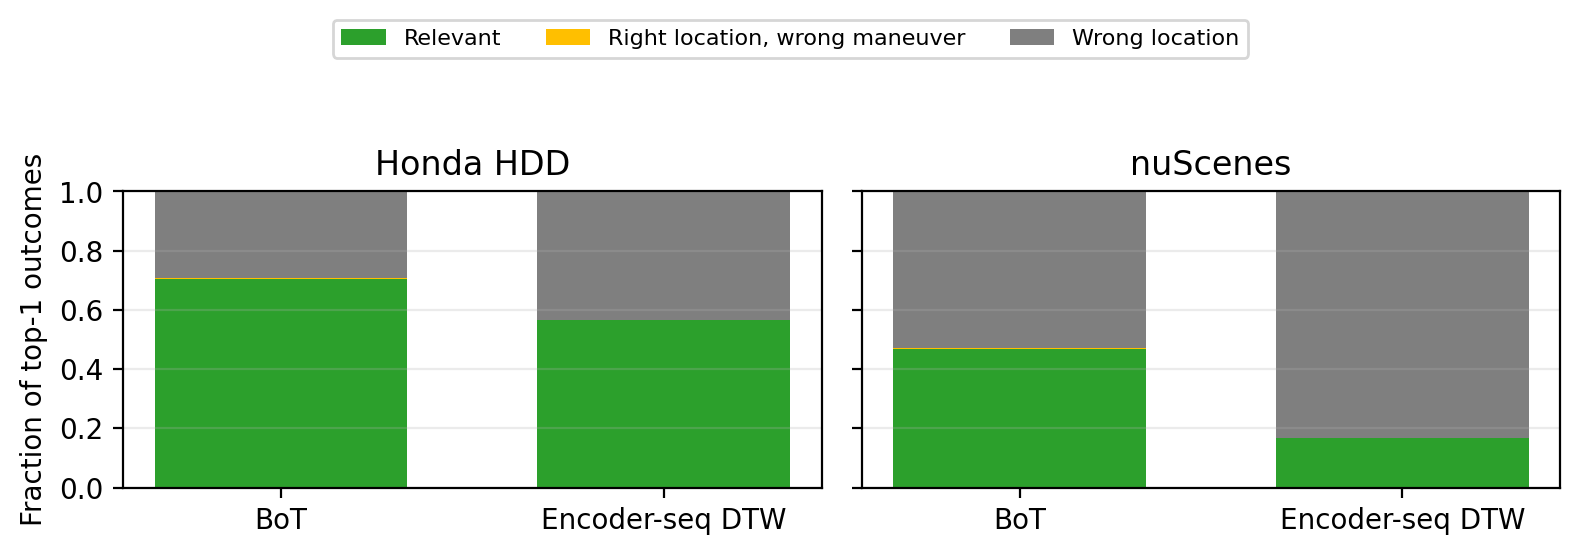
\includegraphics[width=\linewidth]{v4r_error_composition.png}
  \caption{Top-1 outcome composition over the full evaluation gallery. Each retrieved item is
  relevant (same intersection and maneuver), a maneuver error at the correct intersection, or an
  error from a different intersection. This separates conditional maneuver discrimination from
  location discrimination.}
  \label{fig:error_composition}
\end{figure}

We test whether that conditional strength matters for directed retrieval over the full evaluation
galleries of Honda HDD~\cite{honda_hdd} and nuScenes~\cite{nuscenes}. Both sequence comparators lose
globally; a fixed BoT$\to$encoder-sequence-DTW cascade degrades accuracy; and cross-validated score
fusion assigns essentially all weight to appearance. Our contributions are:
\begin{itemize}
  \item A matched query-wise comparison of local and full galleries, with cluster-bootstrap
  uncertainty, on two driving datasets.
  \item Evidence that both sequence comparators improve conditionally yet underperform globally,
  with error decomposition, reranking, and held-out fusion localizing the failure.
  \item Pooled-pair shuffled-order and assignment controls separating intact-order benefits from
  finer per-frame matching.
\end{itemize}
Anonymous code and evaluation artifacts are available online.\footnote{\url{https://anonymous.4open.science/r/diagnosing-temporal-sensitivity-7FD3/}}
Our claims are scoped to these datasets, representations, comparators, and the linear fusion
protocol, not video models in general.

\section{Diagnostics and Protocols}
\label{sec:protocols}
\textbf{Representations and comparators.} V-JEPA~2~\cite{vjepa2} BoT mean-pools contextual tokens
and therefore is not guaranteed to share the exact order invariance of pooled independent-frame features.
We compare it with V-JEPA~2 encoder-sequence DTW and temporal-residual DTW. V-JEPA~2 ingests $64$
frames as $32\times16\times16$ spatiotemporal patches ($D{=}1024$); the encoder sequence
spatially averages patches per temporal position to a $(32, D)$ trajectory, the residual averages
predictor--target differences at each of $16$ target positions, and BoT mean-pools all patch tokens
to one vector.

\textbf{DTW and normalization.} DTW aligns two sequences by a minimum-cost monotonic path that may
stretch but not reverse time. Each sequence and feature dimension is independently min--max
normalized over time; the accumulated path cost is normalized by $T_1{+}T_2$, and similarity is
$\exp(-d_\mathrm{DTW})$. For one distance matrix this transform is monotone, so AP rankings are
invariant to the scale constant while the similarity values are not; scores from different
comparators are therefore not numerically comparable.

\textbf{Segments, clusters, eligibility.} Maneuver segments are grouped into intersections by DBSCAN
on GPS position ($\epsilon{\approx}30$\,m; min.\ samples $3$ for HDD, $2$ for nuScenes); nuScenes
clustering runs independently within each map's local coordinate frame. An
intersection is retained if it contains both left and right turns. A candidate is \emph{relevant} to a query if it shares the
query's intersection cluster \emph{and} maneuver label; out-of-cluster candidates remain negatives.
A segment is an eligible query if it has at least one relevant gallery item. HDD yields $1{,}687$
segments and $1{,}673$ eligible queries in the $50$ largest mixed clusters; nuScenes
(v1.0-trainval) yields $244$ segments from the $50$ largest mixed clusters, with $197$ eligible
queries drawn from $37$ clusters.

\textbf{Directed retrieval and fusion.} Each eligible segment queries either the other retained
segments at its intersection (conditional retrieval) or every other retained segment (global
retrieval). Both use the same eligible queries and report query-macro mAP; global retrieval also
reports mean reciprocal rank (MRR). We test (i) a cascade that reranks the BoT top-$k$ with
encoder-sequence DTW, and (ii) a per-query linear fusion of the same two scores,
$\alpha\,z(\text{BoT}) + (1{-}\alpha)\,z(-d_\mathrm{enc})$, over the valid gallery, where
$d_\mathrm{enc}$ is the encoder-sequence DTW distance.
The weight $\alpha$ is chosen over a $21$-point grid on $[0,1]$ by leave-one-cluster-out
cross-validation: for each held-out intersection, $\alpha$ maximizes mean training-query AP on the
other clusters with the held-out cluster removed from both the tuning queries and their galleries;
ties keep a single maximizing endpoint, else the middle maximizing grid point. The selected
$\alpha$ is then applied to the held-out queries against the \emph{full} gallery, so no query
informs its own weight.

\textbf{Controls and uncertainty.} Primary conditional and global results macro-average per-query
AP over the same eligible query set. Shuffled-DTW and assignment controls instead use a separate
pooled AP protocol over unordered within-cluster pairs: $97{,}731$ from $1{,}687$ HDD segments and
$824$ from $244$ nuScenes segments. All $95\%$ intervals use $2000$ intersection-cluster bootstrap
resamples. We report marginal method intervals and paired difference intervals separately; fusion
intervals bootstrap fixed out-of-fold query metrics rather than refitting $\alpha$ per resample.

\section{Retrieval: Conditional Gains Reverse Globally}
\label{sec:retrieval}
\textbf{Conditional retrieval favors sequence comparison.} Restricting each query to its
intersection, encoder-sequence DTW reaches mAP $0.955$ versus BoT's $0.923$ on HDD and $0.922$
versus $0.855$ on nuScenes (\cref{tab:reversal}, top). Paired gains exclude zero: $+0.032$
$[0.016, 0.042]$ and $+0.067$ $[0.036, 0.101]$, respectively.

\textbf{Intact order is not consistently beneficial under pooled-pair AP.} In this separate control
protocol, shuffled DTW permutes each endpoint in turn and averages the two one-sided distances over
10 draws. Intact encoder-sequence DTW exceeds this control detectably only on nuScenes ($+0.063$ AP,
$95\%$ CI $[0.023, 0.102]$); its HDD interval crosses zero ($[-0.001, 0.054]$), as do both residual
DTW intervals. Order-free one-to-one assignment, which also removes one-to-many warping and endpoint
anchoring, has paired intervals spanning zero in three comparisons and improves nuScenes residual
features ($+0.047$ $[0.017, 0.080]$). The nuScenes contrast is provisional because tiling sparse
$2$\,Hz keyframes to 64 frames introduces artificial repetition whose effect is unknown.

\textbf{The ranking reverses across the evaluation gallery.} Under directed gallery retrieval
(\cref{tab:reversal}, middle) both sequence scores lose in mAP and MRR: BoT reaches mAP $0.256$ /
MRR $0.766$ on HDD and $0.333$ / $0.574$ on nuScenes, while encoder-sequence DTW reaches only
$0.177$ / $0.640$ and $0.159$ / $0.281$. Temporal-residual DTW falls further to $0.164$ / $0.616$
and $0.136$ / $0.253$; its paired mAP deficit to BoT is $-0.091$ $[-0.116, -0.077]$ on HDD and
$-0.196$ $[-0.271, -0.136]$ on nuScenes. The result is consistent with insufficient location
discrimination; we test that explanation by decomposing top-ranked outcomes.

\textbf{Top-1 error decomposition.} \cref{fig:error_composition} separates failures at the
correct intersection from retrievals of the wrong location. Same-intersection/wrong-maneuver
outcomes are at most $0.6\%$ for every top-1 ranking. Encoder-sequence DTW increases wrong-intersection
retrieval over BoT by $+0.142$ $[0.108, 0.187]$ on HDD and $+0.294$ $[0.217, 0.369]$ on
nuScenes; residual DTW increases it by $+0.172$ $[0.137, 0.214]$ and $+0.320$ $[0.241, 0.396]$
(paired cluster bootstrap). Thus the conditional gain does not survive location search:
the global error is overwhelmingly selecting the wrong intersection, not the wrong maneuver at the
right one.

\textbf{Neither encoder-sequence cascade nor held-out fusion recovers the gap.} Reranking the BoT top-$k$ by encoder-sequence DTW
lowers AP at every evaluated $k$ on the same candidate set (recall unchanged; \cref{fig:cascade}).
The held-out BoT/encoder-sequence fusion selects $\alpha^\star{=}0.95$ in all $50$ HDD folds and
$\alpha^\star{=}1.0$ in all $37$ nuScenes folds: on HDD the fused mAP shows no detected gain over
BoT ($+0.001$, $[-0.003, 0.004]$), and on nuScenes it collapses exactly onto BoT (difference $0$).

\begin{table}[t]
  \centering
  \caption{Matched conditional vs.\ global query-wise retrieval (V-JEPA~2).
  Top: within-intersection query-macro mAP (marginal $95\%$ cluster CI). Middle: evaluation-gallery
  mAP / MRR (marginal CI on mAP); held-out BoT/encoder-sequence fusion lists $\alpha^\star$.
  Bottom: \emph{paired} cluster-bootstrap difference intervals, reported separately from single
  methods.}
  \label{tab:reversal}
  \small
  \resizebox{\linewidth}{!}{%
  \begin{tabular}{llcc}
    \toprule
     & & \textbf{Honda HDD} & \textbf{nuScenes} \\
    \midrule
    \multicolumn{4}{l}{\emph{Conditional within-intersection retrieval}, mAP $[95\%$ CI$]$} \\
    & BoT (cosine)          & $0.923$ $[0.900, 0.948]$ & $0.855$ $[0.825, 0.890]$ \\
    & Encoder-seq DTW       & $0.955$ $[0.937, 0.971]$ & $0.922$ $[0.895, 0.951]$ \\
    & Temporal-residual DTW & $0.949$ $[0.931, 0.965]$ & $0.903$ $[0.874, 0.935]$ \\
    \midrule
    \multicolumn{4}{l}{\emph{Global query-wise retrieval}, mAP $[95\%$ CI$]$ / MRR} \\
    & BoT (cosine)          & $0.256$ $[0.218, 0.288]$ / $0.766$ & $0.333$ $[0.271, 0.413]$ / $0.574$ \\
    & Encoder-seq DTW       & $0.177$ $[0.135, 0.212]$ / $0.640$ & $0.159$ $[0.122, 0.204]$ / $0.281$ \\
    & Temporal-residual DTW & $0.164$ $[0.126, 0.194]$ / $0.616$ & $0.136$ $[0.102, 0.177]$ / $0.253$ \\
    & Held-out fusion       & $0.257$ $[0.218, 0.289]$ / $0.770$ & $0.333$ $[0.271, 0.413]$ / $0.574$ \\
    & \quad selected $\alpha^\star$ & $0.95$ (all $50$ folds) & $1.00$ (all $37$ folds) \\
    \midrule
    \multicolumn{4}{l}{\emph{Paired difference} (cluster-bootstrap, $95\%$ CI)} \\
    & Enc-seq DTW $-$ BoT (conditional) & $+0.032$ $[0.016, 0.042]$ & $+0.067$ $[0.036, 0.101]$ \\
    & Enc-seq DTW $-$ BoT (global)      & \hddGlobalDtwBot{}       & $-0.173$ $[-0.240, -0.118]$ \\
    & Residual DTW $-$ BoT (global)     & $-0.091$ $[-0.116, -0.077]$ & $-0.196$ $[-0.271, -0.136]$ \\
    & Fusion $-$ BoT (global)           & $+0.001$ $[-0.003, 0.004]$ & $+0.000$ $[0.000, 0.000]$ \\
    \bottomrule
  \end{tabular}
  }
\end{table}

\begin{figure}[t]
  \centering
  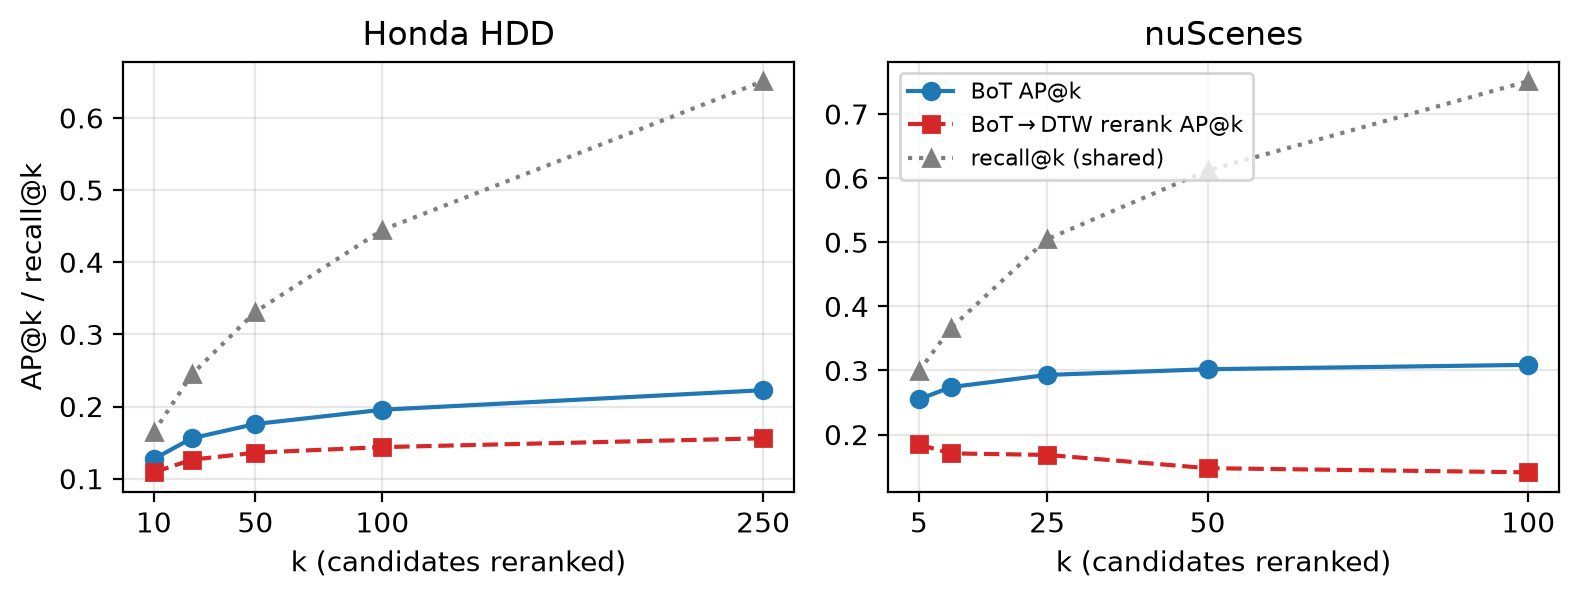
\includegraphics[width=\linewidth]{v4r_cascade.png}
  \caption{BoT$\to$encoder-sequence-DTW cascade. Reranking the BoT top-$k$ lowers AP@$k$ at every evaluated
  $k$ on both datasets; recall@$k$ (shared candidate set) is unchanged.}
  \label{fig:cascade}
\end{figure}

\section{Related Work}
\label{sec:related}
Global video descriptors and pooled matching underpin scalable near-duplicate and event
retrieval~\cite{faiss}, while sequence-alignment comparators such as DTW, Drop-DTW, and temporal
max-similarity capture fine-grained order~\cite{sakoe1978dtw,dropdtw,kordopatis2019visil}. Modern
multi-vector and late-interaction models~\cite{qwen3vlembed} retain finer structure. Our claims
concern pooled global descriptors and the tested DTW variants. The tension between location and
order is closely related to \emph{visual place recognition} (VPR), where global aggregation such as
NetVLAD~\cite{netvlad} enables scalable place matching, and \emph{sequence}-based localization such
as SeqSLAM~\cite{seqslam} and learned sequence descriptors~\cite{seqnet} exploit temporal order
along a route. Our result is a caution for that line: an order-aware sequence score that helps
\emph{within} a place can hurt \emph{across} places if it is not itself place-discriminative.
Temporal analyses commonly use conditional or classification settings
~\cite{lei2022singleframe,tempcompass,temporaltransfer,tracingaot}; our matched galleries expose the
cost of adding location search. Recent theory also bounds what fixed-dimensional embedding rankings
can express~\cite{weller2025limits}, consistent with a temporal score failing to improve an
appearance ranking.

\section{Discussion and Conclusion}
\label{sec:conclusion}
Within-intersection and cross-intersection retrieval measure different capabilities. Sequence
comparators improve conditional matching yet provide too little location discrimination to rank the
evaluation gallery well. The top-1 decomposition localizes the loss to wrong-intersection retrieval;
neither fixed reranking nor a cross-validated linear blend repairs it here. Global sequence retrieval
therefore needs a fine-grained representation that is itself location-discriminative.

\textbf{Deployment and limitations.} BoT supports indexed search; retained-gallery DTW is not
directly indexable and is quadratic in sequence length. The BoT-first cascade bounds DTW work but
reduces accuracy here. The study covers two driving datasets, their $50$ largest mixed-direction
clusters, one backbone, tested DTW variants, and one linear fusion family on a $0.05$ grid.
Per-sequence min--max normalization may itself discard location evidence. Moreover, nuScenes tiles
sparse keyframes to a fixed input length, so its intact-vs-shuffled contrast remains provisional.
These are scoped failure cases, not evidence that sequence retrieval or nonlinear fusion cannot
succeed. We release the diagnostics to support broader tests.

\FloatBarrier

\bibliographystyle{splncs04}
\bibliography{video4real}

\end{document}
